\documentclass{beamer}
\errorcontextlines 1000
\usepackage[utf8]{inputenc}
\usepackage[T1]{fontenc}
\usepackage [italian] {babel}
\usepackage{lmodern}

\usepackage{graphicx}
\usepackage{wrapfig}
\graphicspath{ {immagini/} }

\usepackage{listings}
\renewcommand{\lstlistingname}{Listato}
\renewcommand{\lstlistlistingname}{Elenco dei listati}
\lstset{upquote=true, breaklines=true, columns=flexible}

\usepackage{algorithm}
\usepackage{algorithmicx}
\usepackage{algpseudocode}

\usepackage{caption}
\captionsetup[figure]{labelformat=empty}
\usetheme{Madrid}

\setbeamertemplate{navigation symbols}{}

\title{PyGFA}
\subtitle{Progettazione e sviluppo di una libreria Python per la gestione di file GFA}
\author[Diego Lobba]{Diego Lobba\\
{\footnotesize \textbf{matricola:}795702}}

\institute[Università Milano-Bicocca]{Università degli studi di Milano-Bicocca\\
Dipartimento di Informatica Sistemistica e Comunicazione\\[5pt]
\textbf{Relatore:} {\normalsize Prof. Gianluca Della Vedova}\\
\textbf{Correlatore:} {\normalsize Marco Previtali}}

\date{}

\AtBeginSubsection[]
{
  \begin{frame}<beamer>
    \frametitle{Outline}
    \tableofcontents[
      currentsection,
      sectionstyle=hide,
      subsectionstyle=hide
      ]
  \end{frame}
}

\begin{document}

\begin{frame}
\titlepage
\end{frame}

\section{Attività svolte}
\begin{frame}{\secname}
	\begin{columns}
		\begin{column}{\textwidth}

			\textbf{Motivazioni:}
			\begin{itemize}
				\item Offrire una piattaforma semplice
				\begin{itemize}
					\item da usare
					\item da estendere
				\end{itemize}
				\item Algoritmi per grafi applicati al contesto genomico
			\end{itemize}

			\vspace{10px}

			\textbf{Attività:}
			\begin{itemize}
				\item Studio delle specifiche GFA
				\item Implementazione del sistema
				\item Verifica della correttezza e della qualità
				\item Benchmark per misurare le performance della libreria
			\end{itemize}
		\end{column}
	\end{columns}
\end{frame}

\section{Cos'è il DNA?}
\begin{frame}{\secname}

	\begin{columns}[onlytextwidth]
		\begin{column}{0.6\textwidth}
			\begin{itemize}
				\item DNA come stringa composta dalle lettere A, C, G, T
		    
				\item Stringa ottenuta mediante riassemblaggio di sequenze più piccole
					ottenute da metodi NGS (Next Generation Sequencing)
		    	   
				\item Rappresentare le informazioni di sequenziamento è un problema
			\end{itemize}
		\end{column}    
		
		\begin{column}{0.4\textwidth}
			\begin{figure}
				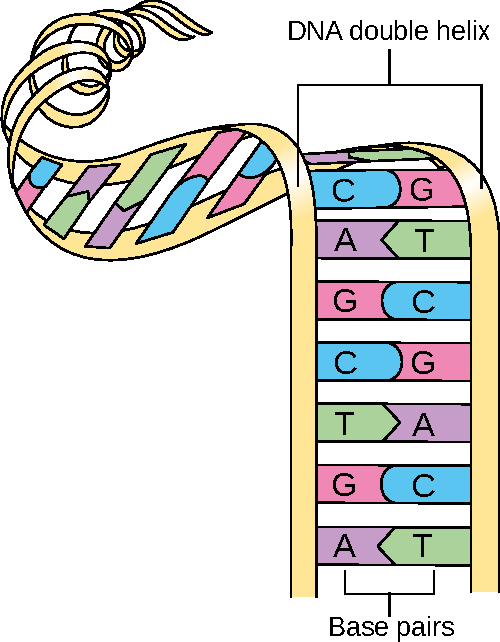
\includegraphics[scale=0.45]{dna}
			\end{figure}
		\end{column}
	\end{columns}
\end{frame}

% -----------------------------------------------------------------------------------------------------------------
 
 \section{I file GFA}
 \begin{frame}[fragile]{\secname}
 	\begin{columns}[b, onlytextwidth]
 		\begin{column}{0.7\textwidth}
 			\begin{itemize}
				\item Due specifiche
					\begin{itemize}
							\item GFA1 pensata appositamente per grafi di assemblaggio
							\item GFA2 più generica, superset di GFA1
					\end{itemize}					
				\item ogni linea rappresenta un concetto
					all'interno del grafo
 			\end{itemize}
 			\begin{figure}
 				\centering
 				\captionsetup{justification=centering}
 				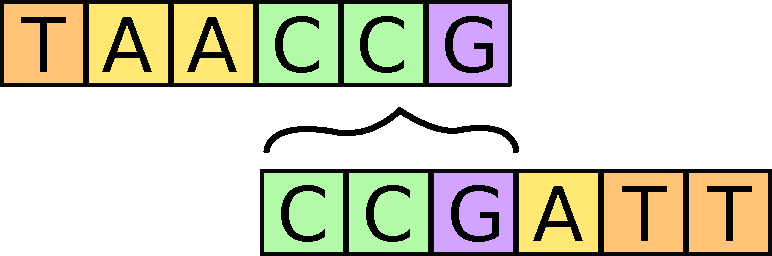
\includegraphics[scale=0.30]{dov_ov_++}
 				\caption{Esempio di sovrapposizione\\a coda di rondine}
 			\end{figure}
 		\end{column}
 		\begin{column}{0.3\textwidth}
 			\begin{figure}
 				\centering
 				\captionsetup{justification=centering}
 				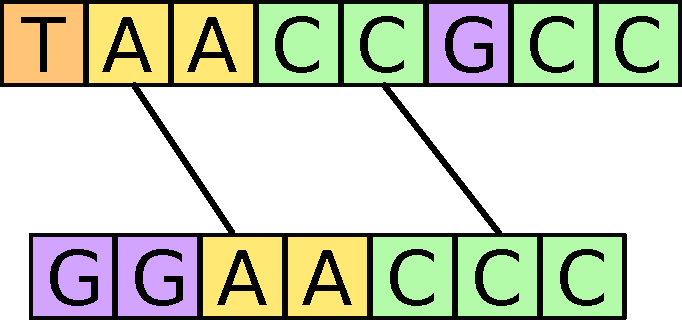
\includegraphics[scale=0.27]{generic-overlap}
 				\caption{Una generica sovrapposizione}
 			\end{figure}
 		\end{column}
 	\end{columns}
 \end{frame}
 
%-------------------------------------------------------------------------------------------------------------------------

\section{PyGFA}
\begin{frame}{\secname}

	\begin{columns}
		\begin{column}{0.7\textwidth}
			\begin{itemize}
				\item \'E una libreria Python
				\item Gestisce le informazioni contenute nei file GFA
				\item Usa la classe \textbf{Multigrafo} offerta da NetworkX per
					contenere le informazioni ed eseguire operazioni
					sul grafo
			\end{itemize}
		\end{column}
		
		\begin{column}{0.3\textwidth}
			\begin{figure}
				
\includegraphics[scale=0.25]{pygfa}
				\caption{Logo di PyGFA.}
			\end{figure}
		\end{column}
		
	\end{columns}
\end{frame}

% ----------------------------------------------------------------------------------------------------------------

\section{Gestione delle informazioni}
\begin{frame}{\secname}
	\begin{columns}
		\begin{column}{0.5\textwidth}
			\begin{itemize}
				\item da linea su file di testo a dizionario Python degli elementi del grafo
				\item gestione particolare degli archi di dovetail
				\item duplice visione del grafo
			\end{itemize}
			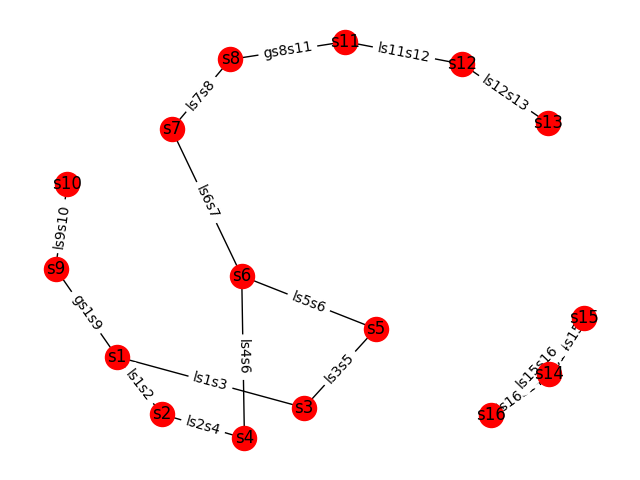
\includegraphics[scale=0.35]{matplot-es}
		\end{column}
		\begin{column}{0.5\textwidth}
			\centering
			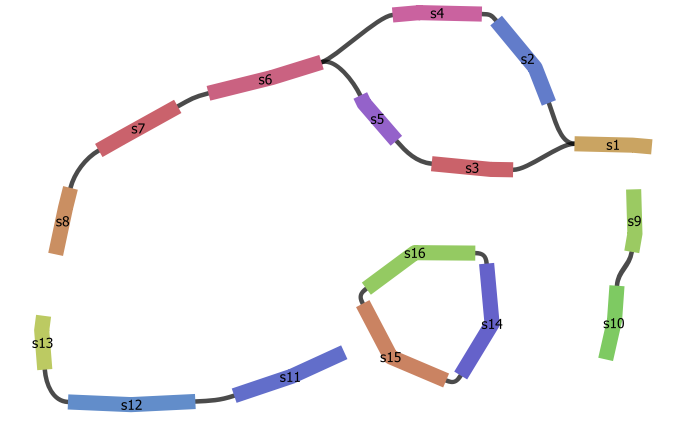
\includegraphics[scale=0.35]{bandage-es}
		\end{column}
	\end{columns}
\end{frame}

% -----------------------------------------------------------------------------------------------------

\section{Funzionalità}
\begin{frame}{\secname}
	\begin{columns}
		\begin{column}{\textwidth}
			\begin{itemize}
				\item calcolo delle componenti connesse
				\item calcolo dei percorsi racchiusi tra due nodi
				\item salvataggio del grafo in una delle due specifiche
				\item ricerca degli elementi del grafo utilizzando un comparatore
					definito dall'utente
			\end{itemize}
		\end{column}
	\end{columns}
\end{frame}

% ---------------------------------------------------------------------------------------------------------

\section{Benchmark}
\begin{frame}{\secname}
	\begin{columns}
		\begin{column}{0.5\textwidth}

			\begin{itemize}
				\item Due serie di test dove:
					\begin{itemize}
						\item si è analizzata la scalabilità di PyGFA
						\item si è confrontata PyGFA con Gfapy
					\end{itemize}
				\item PyGFA ha una grossa occupazione in memoria
				\item A parità di memoria occupata PyGFA è più prestante in termini di tempo
			\end{itemize}

		\end{column}
		\begin{column}{0.5\textwidth}
			\centering
			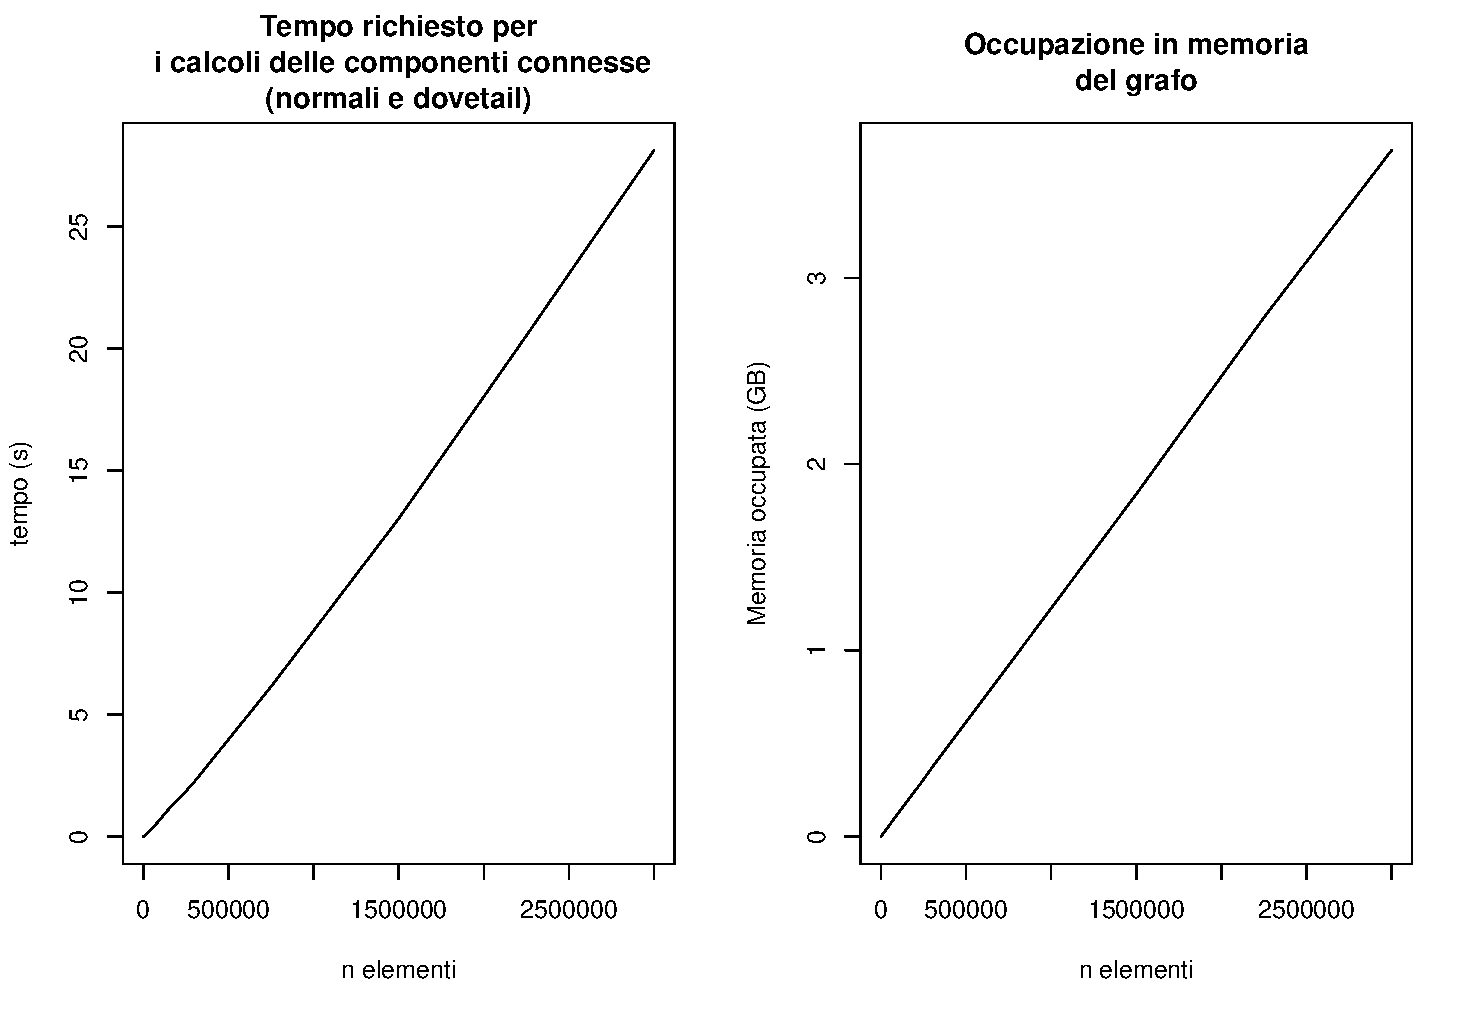
\includegraphics[height=0.45\textheight, width=\textwidth, keepaspectratio]{bench_singular}

			\centering
			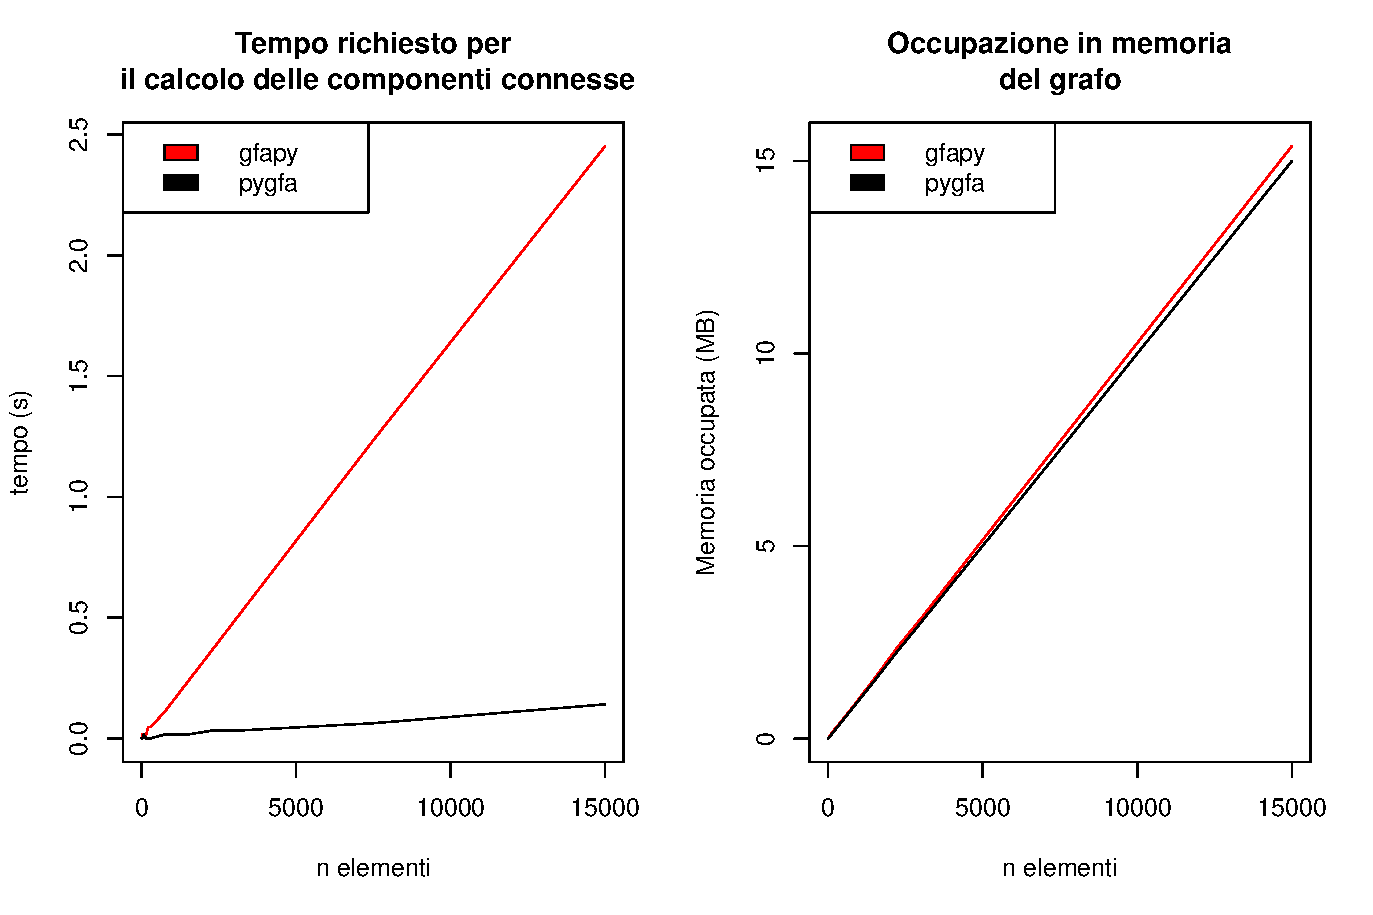
\includegraphics[height=0.45\textheight, width=\textwidth, keepaspectratio]{comparison}
		\end{column}
	\end{columns}
\end{frame}


% ---------------------------------------------------------------------------------------------------------

\section{Confronto delle funzionalità}
\begin{frame}{\secname}
	\begin{columns}[T]
		\begin{column}{0.5\textwidth}
			\textbf{PyGFA:}
			\begin{itemize}
				\item visione astratta dei dati
				\item operazioni su grafo generale
				\item operazioni sul grafo ottenuto considerando
					solo sovrapposizioni a coda di rondine
			\end{itemize}
		\end{column}
		\begin{column}{0.5\textwidth}
			\textbf{Gfapy:}
			\begin{itemize}
				\item il concetto di linea GFA viene mantenuto
				\item fornisce operazioni per grafi di assemblaggio più avanzate
			\end{itemize}
		\end{column}
	\end{columns}
\end{frame}


% --------------------------------------------------------------------------------------------------------------------------

\section[Metodologia e strumenti]{Metodologia e strumenti di aiuto nello sviluppo}
\begin{frame}[fragile]{\secname}
	\begin{columns}
		\begin{column}{0.6\textwidth}
			\textbf{Metodologia:}
			\begin{itemize}

				\item Extreme Programming

				\item Sviluppo basato sulle priorità
					\begin{itemize}
						\item si implementa subito
						\item si implementa affiancati dai casi di test
					\end{itemize}
			\end{itemize}

			\vspace{10px}

			\textbf{Strumenti usati per lo sviluppo:}
			\begin{itemize}
				\item Coverage.py
					\begin{itemize}
						\item copertura dei casi di test
					\end{itemize}
				\item Pylint
				\item Sphinx e Read the Docs
					\begin{itemize}
						\item documentazione autogenerata
						\item output in html con supporto mobile
						\item hosting su piattaforma specifica
					\end{itemize}
			\end{itemize}
		\end{column}
		\begin{column}{0.4\textwidth}
			\begin{flushright}
				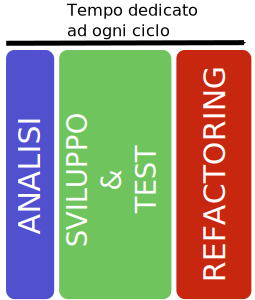
\includegraphics[scale=0.55]{timebox}
			\end{flushright}
		\end{column}
	\end{columns}
\end{frame}

% ---------------------------------------------------------------------------------------------------

\section{Conclusioni}
\begin{frame}{\secname}
	\begin{columns}
		\begin{column}{\textwidth}
			\begin{itemize}
				\item Stato di sviluppo:
					\begin{itemize}
						\item l'attuale versione è stabile
						\item necessità di un refactoring più accurato
						\item piattaforma estendibile
					\end{itemize}
			\end{itemize}
		\end{column}
	\end{columns}
\end{frame}
	
\begin{frame}{}
	\centering
	{\Large{Grazie dell'attenzione!}}
\end{frame}

% DNA, NGS, salvataggio informazioni------------------------------------------------ V
% file GFA - cosa descrivono, motivazioni-------------------------------------------- V
% PyGFA - perchè, cosa fa, cosa usa------------------------------------------------ V
% Gestione delle informazioni, dovetails, doppia visione del grafo e
%		livello di astrazione ------------------------------------------------------------- V
% funzionalità introdotte, problematiche e soluzioni -------------------------------- V
% Benchmark, confronto con gfapy -------------------------------------------------- V
% Metodo di sviluppo (extreme programming), piani di analisi e
%		iterazione------------------------------------------------------------------------- V(?)
% strumenti di aiuto, coverage sphinx, pylint --------------------------------------- V
% FINE


\end{document}